%===================================================================================
% JORNADA CIENTÍFICA ESTUDIANTIL - MATCOM, UH
%===================================================================================
% Esta plantilla ha sido diseñada para ser usada en los artículos de la
% Jornada Científica Estudiantil de MatCom.
%
% Por favor, siga las instrucciones de esta plantilla y rellene en las secciones
% correspondientes.
%
% NOTA: Necesitará el archivo 'jcematcom.sty' en la misma carpeta donde esté este
%       archivo para poder utilizar esta plantila.
%===================================================================================



%===================================================================================
% PREÁMBULO
%-----------------------------------------------------------------------------------
\documentclass[a4paper,10pt,twocolumn]{article}

%===================================================================================
% Paquetes
%-----------------------------------------------------------------------------------
\usepackage{amsmath}
\usepackage{amsfonts}
\usepackage{amssymb}
\usepackage{jcematcom}
\usepackage[utf8]{inputenc}
\usepackage{listings}
\usepackage[pdftex]{hyperref}
\usepackage{caption}
\usepackage{subcaption}
%-----------------------------------------------------------------------------------
% Configuración
%-----------------------------------------------------------------------------------
\hypersetup{colorlinks,%
	    citecolor=black,%
	    filecolor=black,%
	    linkcolor=black,%
	    urlcolor=blue}

%===================================================================================



%===================================================================================
% Presentacion
%-----------------------------------------------------------------------------------
% Título
%-----------------------------------------------------------------------------------
\title{Proyecto final de matemática numérica} 

%-----------------------------------------------------------------------------------
% Autores
%-----------------------------------------------------------------------------------
\author{\\
\name Cristina Hernández Fornaris \email \href{mailto:a.uno@lab.matcom.uh.cu}{a.uno@lab.matcom.uh.cu}
	\\ \addr Grupo D111 \AND
\name Alberto E Marichal Foseca \email \href{mailto:a.dos@lab.matcom.uh.cu}{a.dos@lab.matcom.uh.cu}
  \\ \addr Grupo D111\AND
\name Dalia Castro Valdes \email \href{mailto:a.dos@lab.matcom.uh.cu}{a.dos@lab.matcom.uh.cu}
  \\ \addr Grupo D111}

%-----------------------------------------------------------------------------------
% Tutores
%-----------------------------------------------------------------------------------
\tutors{\\
Dr. Angela, León Mecías \emph{Centro} \\
Lic. Rocío Ortíz Gancedo, \emph{Centro}\\
Lic. Lázaro D González Martínez\emph{Centro}}

%-----------------------------------------------------------------------------------
% Headings
%-----------------------------------------------------------------------------------
\jcematcomheading{\the\year}{1-\pageref{end}}{Cristina, Alberto, Dalia}

%-----------------------------------------------------------------------------------
\ShortHeadings{MN}{Autores}
%===================================================================================



%===================================================================================
% DOCUMENTO
%-----------------------------------------------------------------------------------
\begin{document}

%-----------------------------------------------------------------------------------
% NO BORRAR ESTA LINEA!
%-----------------------------------------------------------------------------------
\twocolumn[
%-----------------------------------------------------------------------------------

\maketitle

%===================================================================================
% Resumen y Abstract
%-----------------------------------------------------------------------------------
\selectlanguage{spanish} % Para producir el documento en Español

%-----------------------------------------------------------------------------------
% Resumen en Español
%-----------------------------------------------------------------------------------
\begin{abstract}

	Este estudio se enfocó en el desarrollo de un modelo predictivo para clasificar tumores mamarios como benignos o malignos. Para ello, se utilizó un dataset con 30 características de 569 personas, junto con su respectiva clasificación. Se aplicaron dos técnicas clave: la Descomposición en Valores Singulares (SVD) y la Regresión Logística (RL). El SVD permitió reducir la dimensionalidad de los datos, identificando que los primeros 4 valores singulares concentraban la mayor parte de la información relevante. Posteriormente, el modelo de Regresión Logística, entrenado con los datos reducidos, mostró una alta exactitud del 94\% en la clasificación de los tumores. La combinación de estos métodos de aprendizaje automático y álgebra lineal demostró ser eficaz para optimizar el procesamiento de datos complejos y mejorar la precisión en la predicción de la naturaleza de los tumores. Los resultados subrayan el potencial de estas técnicas para avanzar en el diagnóstico del cáncer de mama y otros problemas médicos desafiantes. Este enfoque innovador puede contribuir significativamente a una detección temprana más efectiva y a un tratamiento más adecuado de esta enfermedad.

\end{abstract}

%-----------------------------------------------------------------------------------
% English Abstract
%-----------------------------------------------------------------------------------
\vspace{0.5cm}

\begin{enabstract}

 This study focused on developing a predictive model to classify breast tumors as benign or malignant. To do so, a dataset with 30 features from 569 people was used, along with their respective classification. Two key techniques were applied: Singular Value Decomposition (SVD) and Logistic Regression (RL). SVD allowed reducing the dimensionality of the data, identifying that the first 4 singular values ​​concentrated most of the relevant information. Subsequently, the Logistic Regression model, trained with the reduced data, showed a high accuracy of 94\% in classifying tumors.
The combination of these machine learning and linear algebra methods proved to be effective in optimizing the processing of complex data and improving the accuracy in predicting the nature of tumors. The results underline the potential of these techniques to advance the diagnosis of breast cancer and other challenging medical problems. This innovative approach can significantly contribute to more effective early detection and more appropriate treatment of this disease.
\end{enabstract}

%-----------------------------------------------------------------------------------
% Palabras clave
%-----------------------------------------------------------------------------------
\begin{keywords}
	Regresión Logistica (RL),
	Descomposición en Valores Singulares (SVD
\end{keywords}

%-----------------------------------------------------------------------------------
% Temas
%-----------------------------------------------------------------------------------
\begin{topics}
	Cáncer de mama
\end{topics}


%-----------------------------------------------------------------------------------
% NO BORRAR ESTAS LINEAS!
%-----------------------------------------------------------------------------------
\vspace{0.8cm}
]
%-----------------------------------------------------------------------------------


%===================================================================================

%===================================================================================
% Introducción
%-----------------------------------------------------------------------------------
\section{Introducción}\label{sec:intro}
%-----------------------------------------------------------------------------------
  El cáncer de mama se encuentra entre las enfermedades más comunes y complejas de la sociedad contemporánea y afecta a millones de personas en todo el mundo. Es el principal cáncer entre mujeres, lo que lo convierte en un importante problema de salud pública mundial. Así, diferenciar entre tumores benignos y malignos ha adquirido importancia en la detección temprana y el tratamiento eficaz.

Con los avances dados por la tecnología médica y la ciencia de datos en los últimos tiempos, se abren nuevas vías para una mejor detención y procedimientos de estadificación del cáncer de mama, sin los cuales de otro modo no habrían sido posibles.

El uso de algorítmos de aprendizaje autómatico combinados con análisis de big data traerá cambios drásticos con respecto a nuestra capacidad para predecir si los casos detectados probablemente sean benignos o malignos. En última instancia, esto revolucionará significativamente la forma en que abordamos estos casos.

En este estudio nos enfocamos en el desarrolo de un modelo predictivo para clasificar tumores mamarios como benignos o malignos. Para ello utilizaremos un dataset que cuenta con 30 características diferentes, de este tipo de tumor, para 569 personas, junto con su respectiva clasificación en benigno (B) o maligno (M). Aplicaremos dos técnicas de aprendizaje autómatico y Álgebra Lineal: la Descomposición en Valores Singulares (SVD) para reducir la dimensionalidad de los datos y la Regresión Logística (RL) como clasificador binario.

%===================================================================================



%===================================================================================
% Desarrollo
%-----------------------------------------------------------------------------------
\section{Desarrollo}\label{sec:dev}
%-----------------------------------------------------------------------------------
  Para poder analizar el dataset de forma eficiente teníamos que reducir la dimensión de la matriz conformada por sus datos. Es por ello que lo primero que realizamos fue el SVD que permite mediante la descomposición de cualquier matriz A en el producto de tres matrices especiales, obtener otra cuyas dimensiones sean menor que la original y que mantenga la mayor cantidad posible de información relevante.
\[
    A = U \Sigma V^T
\]

\begin{description}
			\item $U_{m \times m} \quad$ Es una matriz ortogonal de vectores singulares izquierdos.[1]
			\item $\Sigma_{m \times n}$ Es una matriz diagonal de valores singulares no negativos y ordenados en forma decreciente. Cada valor singular indica la ”importancia” o el peso de una dimensión en la matriz original. Los valores singulares más grandes representan dimensiones que capturan más varianza de los datos.[1]
            \item $V^T_{n \times n}$ Es una matriz diagonal de valores singulares no negativos y ordenados en forma decreciente[1].\\
		\end{description}

Aplicamos SVD en la matriz de datos y obtuvimos las matrices laterales de la fórmula anterior y un vector que contiene los valores singulares de nuestra matriz. La longitud de este es igual al menor valor entre el número de filas y columnas de A.

Al obtener los valores singulares calculamos la proporción de cada uno en relación con la suma total de todos estos y lo expresamos como un porcentajes para entender cúanta ”varianza” o ”información” aporta cada componente en la descomposición, quedándonos la siguiente lista, donde se observa que en los primeros 4 valores es donde está la mayor cantidad de información.

[87.9866555711066, 7.089033223673957,             2.516334406324024,
1.586524268162142, 0.43767538805754985, 0.16373376174050186,

0.09218159061776625, 0.04158128848753281, 0.028101659978320936,

0.020206004415555937, 0.012647608184517092, 0.00630371598406768,

0.0040273642966775075, 0.003341653887763606, 0.002480985043548252,

0.0017680471749349131, 0.0013568537952639366, 0.0013187633091358917,

0.0009374740915346334, 0.0008788317954237511, 0.0006022566545427467,

0.0005765371960134155, 0.0004026631459955914, 0.000363325919442212,

0.00028179742757554146, 0.00024081026912073028, 0.00016139332976105455,

0.00012707365506786766, 9.644645520411048e-05, 5.9235820488086806e-05]

\begin{figure}
    \centering
    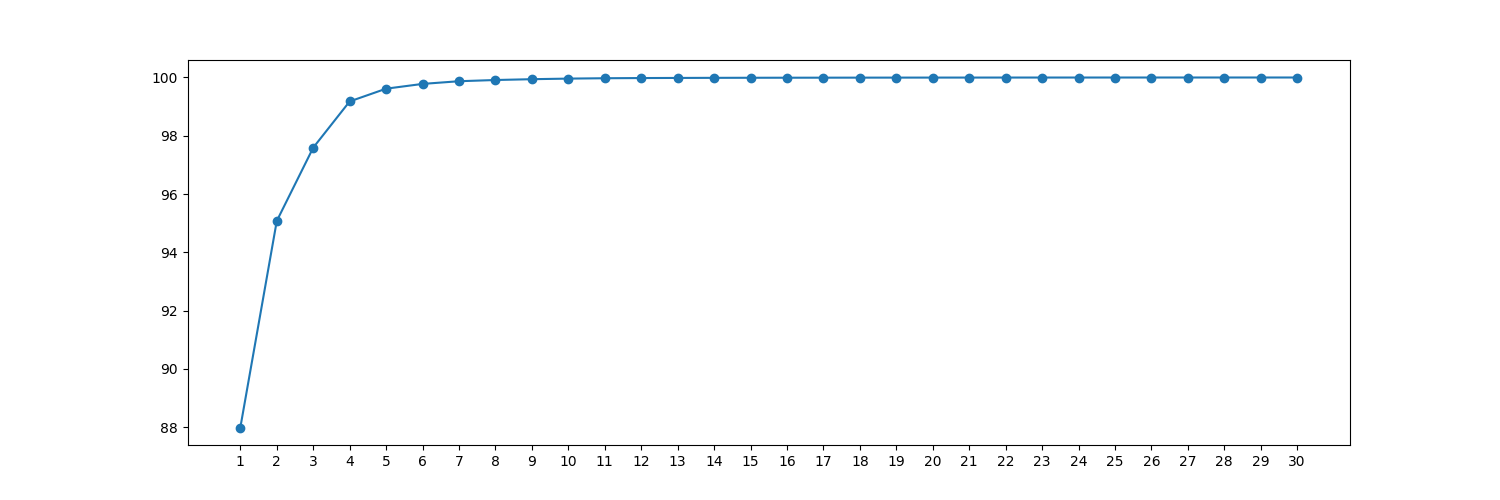
\includegraphics[width=1\linewidth]{svd.png}
    \caption{Porciento de cada valor singular}
    \label{fig:enter-label}
\end{figure}

De esta manera, al probar reducir la dimensionalidad con estos valores identificamos que con k=3 y k=2 obteníamos, al calcular la exactitud del modelo los resultados más precisos. De ahí que escogiéramos k=2, porque al disminuir el número de componentes se reduce la dimensionalidad de los datos, lo que puede mejorar la eficiencia en términos de tiempo de entrenamiento y predicción.

Por tanto se truncó la matriz con k=2 y se aproximó A para ser utilizada en el entrenamiento del modelo de regresión logística.

\[
A \approx U_k \Sigma_k V^*
\]

La Regresión Logística es una técnica estadística utilizada para analizar y modelar la relación entre una variable dependiente categórica (generalmente binaria) y una o más variables independientes.

\[
\sigma(z) = \frac{1}{1 + e^{-z}}
\]
Dónde:
\[
z = \beta_0 + \beta_1 x_1 + \beta_2 x_2 + \cdots + \beta_n x_n 
\]

\textbf{\textit{Modelo de Regresión Logística}}

\[
P(y=1|X) = \beta_0+\beta_1x_1+\beta_2x_2+\dots+\beta_nx_n
\]
Dónde $P(y=1|X)$ es la probabilidad estimada de que la observación pertenezca a la clase positiva.


A continuación dividimos los datos reducidos en conjuntos de entrenamiento y prueba y al calcular el desempeño de del modelo en datos no vistos obtuvimos un 94\% aproximadamente de exactitud.
\section{Conclusiones}
Este estudio ha demostrado la eficacia de combinar técnicas avanzadas de aprendizaje automático y Álgebra Lineal en el análisis de datos médicos. Mediante la aplicación de SVD, logramos reducir la dimensionalidad de un conjunto de datos complejo con 30 características y 569 muestras, manteniendo a mayor parte de la información relevante. Posteriormente, el modelo de regresión logística, entrenado con estos datos reducidos, mostró una alta exactitud del 94\% en la clasificación de tumores. Esta combinación de métodos no solo optimiza el procesamiento de datos, sino que también mejora la precisión en la predicción de la naturaleza de los tumores. Los resultados subrayan el potencial de las técnicas de aprendizaje automático y análisis dimensional en la mejora de las herramientas de diagnóstico, proporcionando un avance significativo en la forma en que abordamos el cáncer de mama y otros problemas médicos complejos.
%-----------------------------------------------------------------------------------
	
%-----------------------------------------------------------------------------------
		
%-----------------------------------------------------------------------------------
	

%===================================================================================



%===================================================================================
% Conclusiones
%-----------------------------------------------------------------------------------

%===================================================================================
% Bibliografía
%-----------------------------------------------------------------------------------
\begin{thebibliography}{99}
%-----------------------------------------------------------------------------------
	\bibitem{luciano} Luciano A Perez. \emph{Descomposici´on SVD.}, 2015.
	\bibitem{goedel} Dimitrios Mitsotakis. B \emph{Computational Mathematics An Introduction to Numerical Analysis and Scientific Computing with Python.}. 2023

	\bibitem{data} Datos. URL: \href{https://www.kaggle.com/datasets/erdemtaha/cancer-data}
{https://www.kaggle.com/datasets/erdemtaha/cancer-data}.
\bibitem{licencia} licencia. URL: \href{https://creativecommons.org/licenses/by-nc-sa/4.0/bajoestalicencia}
{https://creativecommons.org/licenses/by-nc-sa/4.0/bajoestalicencia}.
%-----------------------------------------------------------------------------------
\end{thebibliography}

%-----------------------------------------------------------------------------------

\label{end}

\end{document}

%===================================================================================
